\subsection*{Simple pattern recognition}

This is an academic example defined by a data set with $100$ instances, $2$ inputs, or attributes, and $1$ target. 
The target variable represents two classes ($0$ and $1$). 
The aim is to design a neural network that can predict the correct class for given attribute values. 
Figure \ref{SimplePatternRecognitionFigure} shows this data set.

\begin{figure}[!hbp]
\begin{center}
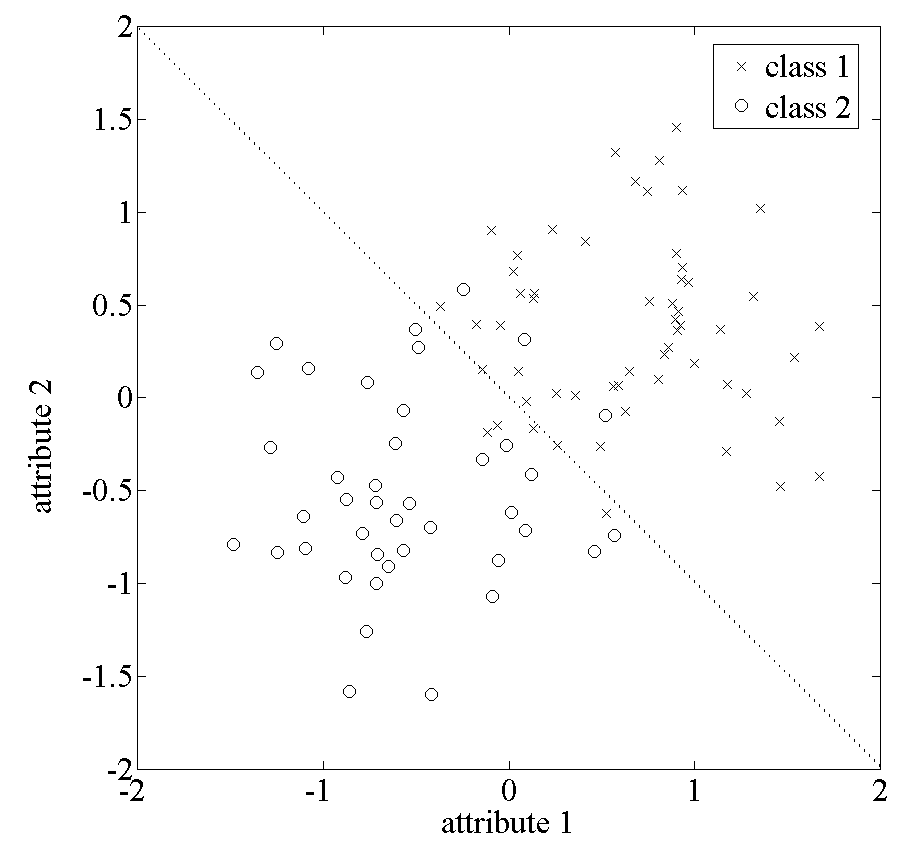
\includegraphics[width=0.75\textwidth]{pattern_recognition/simple_pattern_recognition_data_set.png}
\caption{Data set for the simple pattern recognition example.}\label{SimplePatternRecognitionFigure}
\end{center}
\end{figure}

\subsection*{Iris plant}

This is perhaps the best known data set to be found in the pattern recognition literature. 
It contains $3$ classes of $50$ instances each, where each class refers to a type of iris plant. 
One class is linearly separable from the other two; the latter are not linearly separable from each other.
Figure \ref{IrisPlantFigure} illustrates this example. That picture is has been taken from Wikipedia.  

\begin{figure}[!hbp]
\begin{center}
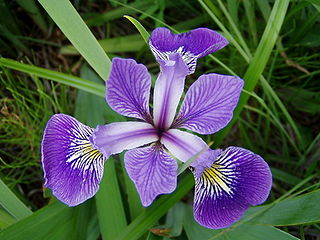
\includegraphics[width=0.6\textwidth]{pattern_recognition/iris_versicolor}
\caption{Iris versicolor.}\label{IrisPlantFigure}
\end{center}
\end{figure}

The input variables are:

\begin{enumerate}
\item Sepal length, in centimeters.
\item Sepal width, in centimeters.
\item Petal length, in centimeters.
\item Petal width, in centimeters.
\item Class -iris setosa, iris versicolour or iris virginica.
\end{enumerate}

The predicted class is the class of iris plant:
 
\begin{enumerate}
\item Iris setosa (true or false).
\item Iris versicolour (true or false).
\item Iris virginica (true or false).
\end{enumerate}

More information on this problem can be found in \cite{UCI}.

\subsection*{Pima indians diabetes}

Pima Indians of Arizona have the population with the highest rate of diabetics in the world. 
It has been estimated that around $50\%$ of adults suffer from this disease. 
The aim of this pattern recognition problem is to predict whether an individual of Pima Indian heritage has diabetes from personal characteristics and physical measurements.
Figure \ref{BloodGlucoseTestingFigure} is a blood glucose testing device, showed here to illustrate this example. 
That picture has been taken from Wikipedia. 

\begin{figure}[!hbp]
\begin{center}
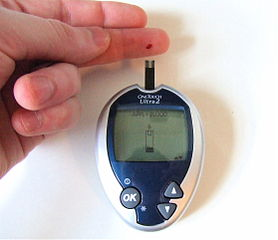
\includegraphics[width=0.5\textwidth]{pattern_recognition/blood_glucose_testing}
\caption{Blood glucose testing.}\label{BloodGlucoseTestingFigure}
\end{center}
\end{figure}


The data is taken from the UCI Machine Learning Repository
\cite{UCI}. The number of samples in the data set is $768$.
The number of input variables for each sample is $8$. All input
variables are numeric-valued, and represent personal
characteristics and physical measurements of an individual. The
number of target variables is $1$, and represents the absence or
presence of diabetes in an individual. Table
\ref{DataSetInformation} summarizes the 
data set information, while tables \ref{InputVariablesInformation}
and \ref{TargetVariablesInformation} depict the input and target
variables information, respectively.

\begin{table}[h!]
\begin{center}
\begin{tabular}{cc}
\hline
Number of instances: & $768$ \\
Number of input variables: & $8$ \\
Number of target variables: & $1$ \\
\hline
\end{tabular}\caption{Data set information.}\label{DataSetInformation}
\end{center}
\end{table}


\begin{table}[h!]
\begin{center}
\begin{tabular}{cc}
\hline
1. & Number of times pregnant.\\
2. & Plasma glucose concentration a 2 hours in an oral glucose tolerance test.\\
3. & Diastolic blood pressure ($mm Hg$).  \\
4. & Triceps skin fold thickness ($mm$).  \\
5. & 2-Hour serum insulin ($mu U/ml$). \\
6. & Body mass index (weight in $kg$/(height in $m$)$^2$). \\
7. & Diabetes pedigree function. \\
8. & Age (years). \\
\hline
\end{tabular}\caption{Input variables information.}\label{InputVariablesInformation}
\end{center}
\end{table}

\begin{table}[h!]
\begin{center}
\begin{tabular}{cc}
\hline
1. & Absence or presence of diabetes (0 or 1). \\
\hline
\end{tabular}\caption{Target variables information.}\label{TargetVariablesInformation}
\end{center}
\end{table}

